\documentclass[1p]{elsarticle_modified}
%\bibliographystyle{elsarticle-num}

%\usepackage[colorlinks]{hyperref}
%\usepackage{abbrmath_seonhwa} %\Abb, \Ascr, \Acal ,\Abf, \Afrak
\usepackage{amsfonts}
\usepackage{amssymb}
\usepackage{amsmath}
\usepackage{amsthm}
\usepackage{scalefnt}
\usepackage{amsbsy}
\usepackage{kotex}
\usepackage{caption}
\usepackage{subfig}
\usepackage{color}
\usepackage{graphicx}
\usepackage{xcolor} %% white, black, red, green, blue, cyan, magenta, yellow
\usepackage{float}
\usepackage{setspace}
\usepackage{hyperref}

\usepackage{tikz}
\usetikzlibrary{arrows}

\usepackage{multirow}
\usepackage{array} % fixed length table
\usepackage{hhline}

%%%%%%%%%%%%%%%%%%%%%
\makeatletter
\renewcommand*\env@matrix[1][\arraystretch]{%
	\edef\arraystretch{#1}%
	\hskip -\arraycolsep
	\let\@ifnextchar\new@ifnextchar
	\array{*\c@MaxMatrixCols c}}
\makeatother %https://tex.stackexchange.com/questions/14071/how-can-i-increase-the-line-spacing-in-a-matrix
%%%%%%%%%%%%%%%

\usepackage[normalem]{ulem}

\newcommand{\msout}[1]{\ifmmode\text{\sout{\ensuremath{#1}}}\else\sout{#1}\fi}
%SOURCE: \msout is \stkout macro in https://tex.stackexchange.com/questions/20609/strikeout-in-math-mode

\newcommand{\cancel}[1]{
	\ifmmode
	{\color{red}\msout{#1}}
	\else
	{\color{red}\sout{#1}}
	\fi
}

\newcommand{\add}[1]{
	{\color{blue}\uwave{#1}}
}

\newcommand{\replace}[2]{
	\ifmmode
	{\color{red}\msout{#1}}{\color{blue}\uwave{#2}}
	\else
	{\color{red}\sout{#1}}{\color{blue}\uwave{#2}}
	\fi
}

\newcommand{\Sol}{\mathcal{S}} %segment
\newcommand{\D}{D} %diagram
\newcommand{\A}{\mathcal{A}} %arc


%%%%%%%%%%%%%%%%%%%%%%%%%%%%%5 test

\def\sl{\operatorname{\textup{SL}}(2,\Cbb)}
\def\psl{\operatorname{\textup{PSL}}(2,\Cbb)}
\def\quan{\mkern 1mu \triangleright \mkern 1mu}

\theoremstyle{definition}
\newtheorem{thm}{Theorem}[section]
\newtheorem{prop}[thm]{Proposition}
\newtheorem{lem}[thm]{Lemma}
\newtheorem{ques}[thm]{Question}
\newtheorem{cor}[thm]{Corollary}
\newtheorem{defn}[thm]{Definition}
\newtheorem{exam}[thm]{Example}
\newtheorem{rmk}[thm]{Remark}
\newtheorem{alg}[thm]{Algorithm}

\newcommand{\I}{\sqrt{-1}}
\begin{document}

%\begin{frontmatter}
%
%\title{Boundary parabolic representations of knots up to 8 crossings}
%
%%% Group authors per affiliation:
%\author{Yunhi Cho} 
%\address{Department of Mathematics, University of Seoul, Seoul, Korea}
%\ead{yhcho@uos.ac.kr}
%
%
%\author{Seonhwa Kim} %\fnref{s_kim}}
%\address{Center for Geometry and Physics, Institute for Basic Science, Pohang, 37673, Korea}
%\ead{ryeona17@ibs.re.kr}
%
%\author{Hyuk Kim}
%\address{Department of Mathematical Sciences, Seoul National University, Seoul 08826, Korea}
%\ead{hyukkim@snu.ac.kr}
%
%\author{Seokbeom Yoon}
%\address{Department of Mathematical Sciences, Seoul National University, Seoul, 08826,  Korea}
%\ead{sbyoon15@snu.ac.kr}
%
%\begin{abstract}
%We find all boundary parabolic representation of knots up to 8 crossings.
%
%\end{abstract}
%\begin{keyword}
%    \MSC[2010] 57M25 
%\end{keyword}
%
%\end{frontmatter}

%\linenumbers
%\tableofcontents
%
\newcommand\colored[1]{\textcolor{white}{\rule[-0.35ex]{0.8em}{1.4ex}}\kern-0.8em\color{red} #1}%
%\newcommand\colored[1]{\textcolor{white}{ #1}\kern-2.17ex	\textcolor{white}{ #1}\kern-1.81ex	\textcolor{white}{ #1}\kern-2.15ex\color{red}#1	}

{\Large $\underline{12a_{1008}~(K12a_{1008})}$}

\setlength{\tabcolsep}{10pt}
\renewcommand{\arraystretch}{1.6}
\vspace{1cm}\begin{tabular}{m{100pt}>{\centering\arraybackslash}m{274pt}}
\multirow{5}{120pt}{
	\centering
	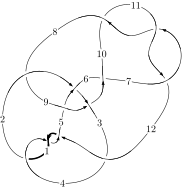
\includegraphics[width=112pt]{../../../GIT/diagram.site/Diagrams/png/1809_12a_1008.png}\\
\ \ \ A knot diagram\footnotemark}&
\allowdisplaybreaks
\textbf{Linearized knot diagam} \\
\cline{2-2}
 &
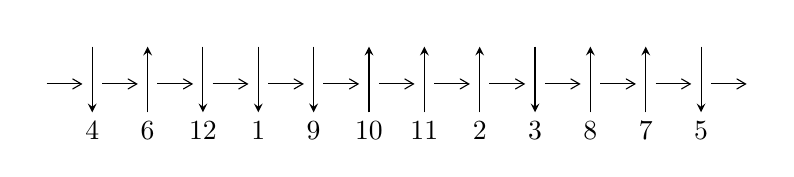
\begin{tikzpicture}[x=20pt, y=17pt]
	% nodes
	\node (C0) at (0, 0) {};
	\node (C1) at (1, 0) {};
	\node (C1U) at (1, +1) {};
	\node (C1D) at (1, -1) {4};

	\node (C2) at (2, 0) {};
	\node (C2U) at (2, +1) {};
	\node (C2D) at (2, -1) {6};

	\node (C3) at (3, 0) {};
	\node (C3U) at (3, +1) {};
	\node (C3D) at (3, -1) {12};

	\node (C4) at (4, 0) {};
	\node (C4U) at (4, +1) {};
	\node (C4D) at (4, -1) {1};

	\node (C5) at (5, 0) {};
	\node (C5U) at (5, +1) {};
	\node (C5D) at (5, -1) {9};

	\node (C6) at (6, 0) {};
	\node (C6U) at (6, +1) {};
	\node (C6D) at (6, -1) {10};

	\node (C7) at (7, 0) {};
	\node (C7U) at (7, +1) {};
	\node (C7D) at (7, -1) {11};

	\node (C8) at (8, 0) {};
	\node (C8U) at (8, +1) {};
	\node (C8D) at (8, -1) {2};

	\node (C9) at (9, 0) {};
	\node (C9U) at (9, +1) {};
	\node (C9D) at (9, -1) {3};

	\node (C10) at (10, 0) {};
	\node (C10U) at (10, +1) {};
	\node (C10D) at (10, -1) {8};

	\node (C11) at (11, 0) {};
	\node (C11U) at (11, +1) {};
	\node (C11D) at (11, -1) {7};

	\node (C12) at (12, 0) {};
	\node (C12U) at (12, +1) {};
	\node (C12D) at (12, -1) {5};
	\node (C13) at (13, 0) {};

	% arrows
	\draw[->,>={angle 60}]
	(C0) edge (C1) (C1) edge (C2) (C2) edge (C3) (C3) edge (C4) (C4) edge (C5) (C5) edge (C6) (C6) edge (C7) (C7) edge (C8) (C8) edge (C9) (C9) edge (C10) (C10) edge (C11) (C11) edge (C12) (C12) edge (C13) ;	\draw[->,>=stealth]
	(C1U) edge (C1D) (C2D) edge (C2U) (C3U) edge (C3D) (C4U) edge (C4D) (C5U) edge (C5D) (C6D) edge (C6U) (C7D) edge (C7U) (C8D) edge (C8U) (C9U) edge (C9D) (C10D) edge (C10U) (C11D) edge (C11U) (C12U) edge (C12D) ;
	\end{tikzpicture} \\
\hhline{~~} \\& 
\textbf{Solving Sequence} \\ \cline{2-2} 
 &
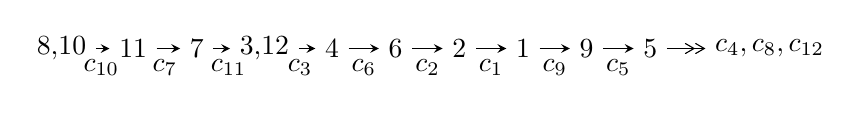
\begin{tikzpicture}[x=23pt, y=7pt]
	% node
	\node (A0) at (-1/8, 0) {8,10};
	\node (A1) at (1, 0) {11};
	\node (A2) at (2, 0) {7};
	\node (A3) at (49/16, 0) {3,12};
	\node (A4) at (33/8, 0) {4};
	\node (A5) at (41/8, 0) {6};
	\node (A6) at (49/8, 0) {2};
	\node (A7) at (57/8, 0) {1};
	\node (A8) at (65/8, 0) {9};
	\node (A9) at (73/8, 0) {5};
	\node (C1) at (1/2, -1) {$c_{10}$};
	\node (C2) at (3/2, -1) {$c_{7}$};
	\node (C3) at (5/2, -1) {$c_{11}$};
	\node (C4) at (29/8, -1) {$c_{3}$};
	\node (C5) at (37/8, -1) {$c_{6}$};
	\node (C6) at (45/8, -1) {$c_{2}$};
	\node (C7) at (53/8, -1) {$c_{1}$};
	\node (C8) at (61/8, -1) {$c_{9}$};
	\node (C9) at (69/8, -1) {$c_{5}$};
	\node (A10) at (11, 0) {$c_{4},c_{8},c_{12}$};

	% edge
	\draw[->,>=stealth]	
	(A0) edge (A1) (A1) edge (A2) (A2) edge (A3) (A3) edge (A4) (A4) edge (A5) (A5) edge (A6) (A6) edge (A7) (A7) edge (A8) (A8) edge (A9) ;
	\draw[->>,>={angle 60}]	
	(A9) edge (A10);
\end{tikzpicture} \\ 

\end{tabular} \\

\footnotetext{
The image of knot diagram is generated by the software ``\textbf{Draw programme}" developed by Andrew Bartholomew(\url{http://www.layer8.co.uk/maths/draw/index.htm\#Running-draw}), where we modified some parts for our purpose(\url{https://github.com/CATsTAILs/LinksPainter}).
}\phantom \\ \newline 
\centering \textbf{Ideals for irreducible components\footnotemark of $X_{\text{par}}$} 
 
\begin{align*}
I^u_{1}&=\langle 
-1.74164\times10^{99} u^{97}-2.39833\times10^{99} u^{96}+\cdots+5.41171\times10^{99} b-4.92742\times10^{99},\\
\phantom{I^u_{1}}&\phantom{= \langle  }-1.17514\times10^{100} u^{97}-1.21460\times10^{100} u^{96}+\cdots+1.62351\times10^{100} a-3.33497\times10^{100},\;u^{98}+u^{97}+\cdots+7 u+1\rangle \\
\\
\end{align*}
\raggedright * 1 irreducible components of $\dim_{\mathbb{C}}=0$, with total 98 representations.\\
\footnotetext{All coefficients of polynomials are rational numbers. But the coefficients are sometimes approximated in decimal forms when there is not enough margin.}
\newpage
\renewcommand{\arraystretch}{1}
\centering \section*{I. $I^u_{1}= \langle -1.74\times10^{99} u^{97}-2.40\times10^{99} u^{96}+\cdots+5.41\times10^{99} b-4.93\times10^{99},\;-1.18\times10^{100} u^{97}-1.21\times10^{100} u^{96}+\cdots+1.62\times10^{100} a-3.33\times10^{100},\;u^{98}+u^{97}+\cdots+7 u+1 \rangle$}
\flushleft \textbf{(i) Arc colorings}\\
\begin{tabular}{m{7pt} m{180pt} m{7pt} m{180pt} }
\flushright $a_{8}=$&$\begin{pmatrix}0\\u\end{pmatrix}$ \\
\flushright $a_{10}=$&$\begin{pmatrix}1\\0\end{pmatrix}$ \\
\flushright $a_{11}=$&$\begin{pmatrix}1\\- u^2\end{pmatrix}$ \\
\flushright $a_{7}=$&$\begin{pmatrix}- u\\u^3+u\end{pmatrix}$ \\
\flushright $a_{3}=$&$\begin{pmatrix}0.723826 u^{97}+0.748131 u^{96}+\cdots+9.72154 u+2.05417\\0.321828 u^{97}+0.443174 u^{96}+\cdots+2.19227 u+0.910511\end{pmatrix}$ \\
\flushright $a_{12}=$&$\begin{pmatrix}u^2+1\\- u^4-2 u^2\end{pmatrix}$ \\
\flushright $a_{4}=$&$\begin{pmatrix}0.277264 u^{97}+0.211124 u^{96}+\cdots+0.311999 u-0.131270\\0.341983 u^{97}+0.481916 u^{96}+\cdots+2.95324 u+1.11161\end{pmatrix}$ \\
\flushright $a_{6}=$&$\begin{pmatrix}- u^3-2 u\\u^3+u\end{pmatrix}$ \\
\flushright $a_{2}=$&$\begin{pmatrix}0.584829 u^{97}+0.589965 u^{96}+\cdots+8.85637 u+1.69336\\0.177735 u^{97}+0.401736 u^{96}+\cdots+2.77552 u+1.13266\end{pmatrix}$ \\
\flushright $a_{1}=$&$\begin{pmatrix}0.114232 u^{97}+0.167614 u^{96}+\cdots-6.85932 u+0.337484\\0.558912 u^{97}+0.496393 u^{96}+\cdots+2.96597 u+0.396995\end{pmatrix}$ \\
\flushright $a_{9}=$&$\begin{pmatrix}0.372776 u^{97}+0.474477 u^{96}+\cdots-13.0178 u-2.46360\\0.0439798 u^{97}-0.196807 u^{96}+\cdots+8.61268 u+0.546451\end{pmatrix}$ \\
\flushright $a_{5}=$&$\begin{pmatrix}-0.188677 u^{97}-0.176374 u^{96}+\cdots-10.6917 u-1.81247\\-0.102684 u^{97}+0.00278592 u^{96}+\cdots+5.61235 u+0.465124\end{pmatrix}$\\&\end{tabular}
\flushleft \textbf{(ii) Obstruction class $= -1$}\\~\\
\flushleft \textbf{(iii) Cusp Shapes $= 3.08296 u^{97}+2.89378 u^{96}+\cdots-32.7657 u-10.5076$}\\~\\
\newpage\renewcommand{\arraystretch}{1}
\flushleft \textbf{(iv) u-Polynomials at the component}\newline \\
\begin{tabular}{m{50pt}|m{274pt}}
Crossings & \hspace{64pt}u-Polynomials at each crossing \\
\hline $$\begin{aligned}c_{1},c_{4},c_{12}\end{aligned}$$&$\begin{aligned}
&u^{98}- u^{97}+\cdots-7 u+1
\end{aligned}$\\
\hline $$\begin{aligned}c_{2}\end{aligned}$$&$\begin{aligned}
&u^{98}-7 u^{97}+\cdots- u+1
\end{aligned}$\\
\hline $$\begin{aligned}c_{3}\end{aligned}$$&$\begin{aligned}
&u^{98}+u^{97}+\cdots-1473 u+2657
\end{aligned}$\\
\hline $$\begin{aligned}c_{5}\end{aligned}$$&$\begin{aligned}
&u^{98}+7 u^{97}+\cdots+u+1
\end{aligned}$\\
\hline $$\begin{aligned}c_{6}\end{aligned}$$&$\begin{aligned}
&u^{98}- u^{97}+\cdots+1473 u+2657
\end{aligned}$\\
\hline $$\begin{aligned}c_{7},c_{10},c_{11}\end{aligned}$$&$\begin{aligned}
&u^{98}+u^{97}+\cdots+7 u+1
\end{aligned}$\\
\hline $$\begin{aligned}c_{8}\end{aligned}$$&$\begin{aligned}
&u^{98}- u^{97}+\cdots+35 u+1
\end{aligned}$\\
\hline $$\begin{aligned}c_{9}\end{aligned}$$&$\begin{aligned}
&u^{98}+u^{97}+\cdots-35 u+1
\end{aligned}$\\
\hline
\end{tabular}\\~\\
\newpage\renewcommand{\arraystretch}{1}
\flushleft \textbf{(v) Riley Polynomials at the component}\newline \\
\begin{tabular}{m{50pt}|m{274pt}}
Crossings & \hspace{64pt}Riley Polynomials at each crossing \\
\hline $$\begin{aligned}c_{1},c_{4},c_{7}\\c_{10},c_{11},c_{12}\end{aligned}$$&$\begin{aligned}
&y^{98}+85 y^{97}+\cdots-7 y+1
\end{aligned}$\\
\hline $$\begin{aligned}c_{2},c_{5}\end{aligned}$$&$\begin{aligned}
&y^{98}-7 y^{97}+\cdots-7 y+1
\end{aligned}$\\
\hline $$\begin{aligned}c_{3},c_{6}\end{aligned}$$&$\begin{aligned}
&y^{98}-23 y^{97}+\cdots+268190649 y+7059649
\end{aligned}$\\
\hline $$\begin{aligned}c_{8},c_{9}\end{aligned}$$&$\begin{aligned}
&y^{98}+109 y^{97}+\cdots+105 y+1
\end{aligned}$\\
\hline
\end{tabular}\\~\\
\newpage\flushleft \textbf{(vi) Complex Volumes and Cusp Shapes}
$$\begin{array}{c|c|c}  
\text{Solutions to }I^u_{1}& \I (\text{vol} + \sqrt{-1}CS) & \text{Cusp shape}\\
 \hline 
\begin{aligned}
u &= -0.491853 + 0.893635 I \\
a &= -1.072020 + 0.324278 I \\
b &= \phantom{-}0.929642 - 1.042110 I\end{aligned}
 & \phantom{-}3.33970 + 9.01230 I & \phantom{-0.000000 } 0 \\ \hline\begin{aligned}
u &= -0.491853 - 0.893635 I \\
a &= -1.072020 - 0.324278 I \\
b &= \phantom{-}0.929642 + 1.042110 I\end{aligned}
 & \phantom{-}3.33970 - 9.01230 I & \phantom{-0.000000 } 0 \\ \hline\begin{aligned}
u &= -0.444484 + 0.841841 I \\
a &= \phantom{-}0.894161 - 0.134799 I \\
b &= -0.867284 + 0.915723 I\end{aligned}
 & -1.86918 + 5.22735 I & \phantom{-0.000000 } 0 \\ \hline\begin{aligned}
u &= -0.444484 - 0.841841 I \\
a &= \phantom{-}0.894161 + 0.134799 I \\
b &= -0.867284 - 0.915723 I\end{aligned}
 & -1.86918 - 5.22735 I & \phantom{-0.000000 } 0 \\ \hline\begin{aligned}
u &= \phantom{-}0.925739 + 0.132292 I \\
a &= \phantom{-}0.615421 + 0.470349 I \\
b &= -0.146037 - 0.355716 I\end{aligned}
 & \phantom{-}6.47609 - 2.18771 I & \phantom{-0.000000 } 0 \\ \hline\begin{aligned}
u &= \phantom{-}0.925739 - 0.132292 I \\
a &= \phantom{-}0.615421 - 0.470349 I \\
b &= -0.146037 + 0.355716 I\end{aligned}
 & \phantom{-}6.47609 + 2.18771 I & \phantom{-0.000000 } 0 \\ \hline\begin{aligned}
u &= \phantom{-}0.859784 + 0.362587 I \\
a &= -0.488034 - 1.051690 I \\
b &= -0.031553 + 0.814056 I\end{aligned}
 & \phantom{-}6.05540 + 4.75636 I & \phantom{-0.000000 } 0 \\ \hline\begin{aligned}
u &= \phantom{-}0.859784 - 0.362587 I \\
a &= -0.488034 + 1.051690 I \\
b &= -0.031553 - 0.814056 I\end{aligned}
 & \phantom{-}6.05540 - 4.75636 I & \phantom{-0.000000 } 0 \\ \hline\begin{aligned}
u &= \phantom{-}0.615615 + 0.643904 I \\
a &= -0.194810 - 0.998527 I \\
b &= -0.344505 + 0.869009 I\end{aligned}
 & \phantom{-}5.01703 + 0.24238 I & \phantom{-0.000000 } 0 \\ \hline\begin{aligned}
u &= \phantom{-}0.615615 - 0.643904 I \\
a &= -0.194810 + 0.998527 I \\
b &= -0.344505 - 0.869009 I\end{aligned}
 & \phantom{-}5.01703 - 0.24238 I & \phantom{-0.000000 } 0\\
 \hline 
 \end{array}$$\newpage$$\begin{array}{c|c|c}  
\text{Solutions to }I^u_{1}& \I (\text{vol} + \sqrt{-1}CS) & \text{Cusp shape}\\
 \hline 
\begin{aligned}
u &= \phantom{-}0.404108 + 1.039140 I \\
a &= \phantom{-}0.131418 - 0.338902 I \\
b &= -0.282590 + 0.595738 I\end{aligned}
 & -1.20967 + 4.26417 I & \phantom{-0.000000 } 0 \\ \hline\begin{aligned}
u &= \phantom{-}0.404108 - 1.039140 I \\
a &= \phantom{-}0.131418 + 0.338902 I \\
b &= -0.282590 - 0.595738 I\end{aligned}
 & -1.20967 - 4.26417 I & \phantom{-0.000000 } 0 \\ \hline\begin{aligned}
u &= -0.324321 + 1.086230 I \\
a &= \phantom{-}0.378494 - 0.891205 I \\
b &= -0.476957 + 1.108320 I\end{aligned}
 & \phantom{-}6.66619 + 0.28302 I & \phantom{-0.000000 } 0 \\ \hline\begin{aligned}
u &= -0.324321 - 1.086230 I \\
a &= \phantom{-}0.378494 + 0.891205 I \\
b &= -0.476957 - 1.108320 I\end{aligned}
 & \phantom{-}6.66619 - 0.28302 I & \phantom{-0.000000 } 0 \\ \hline\begin{aligned}
u &= -0.823277 + 0.259534 I \\
a &= \phantom{-}0.51125 + 2.25920 I \\
b &= -1.07954 - 1.22599 I\end{aligned}
 & \phantom{-}5.3291 - 13.6594 I & \phantom{-}4.15756 + 8.91846 I \\ \hline\begin{aligned}
u &= -0.823277 - 0.259534 I \\
a &= \phantom{-}0.51125 - 2.25920 I \\
b &= -1.07954 + 1.22599 I\end{aligned}
 & \phantom{-}5.3291 + 13.6594 I & \phantom{-}4.15756 - 8.91846 I \\ \hline\begin{aligned}
u &= \phantom{-}0.529507 + 1.014770 I \\
a &= -0.296000 + 0.544554 I \\
b &= \phantom{-}0.462969 - 0.589380 I\end{aligned}
 & \phantom{-}3.75109 + 7.28743 I & \phantom{-0.000000 } 0 \\ \hline\begin{aligned}
u &= \phantom{-}0.529507 - 1.014770 I \\
a &= -0.296000 - 0.544554 I \\
b &= \phantom{-}0.462969 + 0.589380 I\end{aligned}
 & \phantom{-}3.75109 - 7.28743 I & \phantom{-0.000000 } 0 \\ \hline\begin{aligned}
u &= -0.791041 + 0.262127 I \\
a &= -0.45282 - 2.07274 I \\
b &= \phantom{-}1.06829 + 1.10332 I\end{aligned}
 & \phantom{-0.000000 } -9.63418 I & \phantom{-0.000000 -}0. + 8.34982 I \\ \hline\begin{aligned}
u &= -0.791041 - 0.262127 I \\
a &= -0.45282 + 2.07274 I \\
b &= \phantom{-}1.06829 - 1.10332 I\end{aligned}
 & \phantom{-0.000000 -}9.63418 I & \phantom{-0.000000 } 0. - 8.34982 I\\
 \hline 
 \end{array}$$\newpage$$\begin{array}{c|c|c}  
\text{Solutions to }I^u_{1}& \I (\text{vol} + \sqrt{-1}CS) & \text{Cusp shape}\\
 \hline 
\begin{aligned}
u &= -0.041265 + 0.825235 I \\
a &= \phantom{-}0.111753 + 0.211346 I \\
b &= \phantom{-}0.433665 - 0.812752 I\end{aligned}
 & -0.00404 + 1.44418 I & \phantom{-}1.13532 - 1.46067 I \\ \hline\begin{aligned}
u &= -0.041265 - 0.825235 I \\
a &= \phantom{-}0.111753 - 0.211346 I \\
b &= \phantom{-}0.433665 + 0.812752 I\end{aligned}
 & -0.00404 - 1.44418 I & \phantom{-}1.13532 + 1.46067 I \\ \hline\begin{aligned}
u &= \phantom{-}0.737032 + 0.343671 I \\
a &= \phantom{-}0.332554 + 1.052110 I \\
b &= \phantom{-}0.186303 - 0.768333 I\end{aligned}
 & \phantom{-}1.23192 + 2.00806 I & \phantom{-}5.65102 - 9.68372 I \\ \hline\begin{aligned}
u &= \phantom{-}0.737032 - 0.343671 I \\
a &= \phantom{-}0.332554 - 1.052110 I \\
b &= \phantom{-}0.186303 + 0.768333 I\end{aligned}
 & \phantom{-}1.23192 - 2.00806 I & \phantom{-}5.65102 + 9.68372 I \\ \hline\begin{aligned}
u &= -0.126983 + 1.213760 I \\
a &= \phantom{-}1.68278 - 0.99045 I \\
b &= -0.0803647 - 0.0485501 I\end{aligned}
 & \phantom{-}1.53901 + 3.15170 I & \phantom{-0.000000 } 0 \\ \hline\begin{aligned}
u &= -0.126983 - 1.213760 I \\
a &= \phantom{-}1.68278 + 0.99045 I \\
b &= -0.0803647 + 0.0485501 I\end{aligned}
 & \phantom{-}1.53901 - 3.15170 I & \phantom{-0.000000 } 0 \\ \hline\begin{aligned}
u &= -0.740426 + 0.239849 I \\
a &= \phantom{-}0.21070 + 1.84366 I \\
b &= -0.964592 - 0.936497 I\end{aligned}
 & \phantom{-}1.86918 - 5.22735 I & \phantom{-}2.60772 + 4.54430 I \\ \hline\begin{aligned}
u &= -0.740426 - 0.239849 I \\
a &= \phantom{-}0.21070 - 1.84366 I \\
b &= -0.964592 + 0.936497 I\end{aligned}
 & \phantom{-}1.86918 + 5.22735 I & \phantom{-}2.60772 - 4.54430 I \\ \hline\begin{aligned}
u &= -0.763529 + 0.134041 I \\
a &= \phantom{-}0.29520 - 2.22646 I \\
b &= \phantom{-}0.589019 + 1.029750 I\end{aligned}
 & \phantom{-}9.55575 - 4.27219 I & \phantom{-}8.58109 + 5.06376 I \\ \hline\begin{aligned}
u &= -0.763529 - 0.134041 I \\
a &= \phantom{-}0.29520 + 2.22646 I \\
b &= \phantom{-}0.589019 - 1.029750 I\end{aligned}
 & \phantom{-}9.55575 + 4.27219 I & \phantom{-}8.58109 - 5.06376 I\\
 \hline 
 \end{array}$$\newpage$$\begin{array}{c|c|c}  
\text{Solutions to }I^u_{1}& \I (\text{vol} + \sqrt{-1}CS) & \text{Cusp shape}\\
 \hline 
\begin{aligned}
u &= \phantom{-}0.759398 + 0.065192 I \\
a &= \phantom{-}0.072398 - 0.348855 I \\
b &= -0.325726 + 0.222097 I\end{aligned}
 & \phantom{-}1.79931 + 0.03648 I & \phantom{-}7.92424 + 1.99664 I \\ \hline\begin{aligned}
u &= \phantom{-}0.759398 - 0.065192 I \\
a &= \phantom{-}0.072398 + 0.348855 I \\
b &= -0.325726 - 0.222097 I\end{aligned}
 & \phantom{-}1.79931 - 0.03648 I & \phantom{-}7.92424 - 1.99664 I \\ \hline\begin{aligned}
u &= \phantom{-}0.214822 + 1.254110 I \\
a &= \phantom{-}2.41307 + 0.74573 I \\
b &= -0.01191 - 2.30223 I\end{aligned}
 & \phantom{-}0.711582 - 0.106264 I & \phantom{-0.000000 } 0 \\ \hline\begin{aligned}
u &= \phantom{-}0.214822 - 1.254110 I \\
a &= \phantom{-}2.41307 - 0.74573 I \\
b &= -0.01191 + 2.30223 I\end{aligned}
 & \phantom{-}0.711582 + 0.106264 I & \phantom{-0.000000 } 0 \\ \hline\begin{aligned}
u &= \phantom{-}0.179533 + 1.301260 I \\
a &= -1.64385 - 0.90921 I \\
b &= -0.86058 + 1.67816 I\end{aligned}
 & -3.90106 + 2.22326 I & \phantom{-0.000000 } 0 \\ \hline\begin{aligned}
u &= \phantom{-}0.179533 - 1.301260 I \\
a &= -1.64385 + 0.90921 I \\
b &= -0.86058 - 1.67816 I\end{aligned}
 & -3.90106 - 2.22326 I & \phantom{-0.000000 } 0 \\ \hline\begin{aligned}
u &= -0.130364 + 1.321870 I \\
a &= \phantom{-}0.694450 + 0.523183 I \\
b &= \phantom{-}0.912458 - 0.693022 I\end{aligned}
 & -2.06229 + 2.57316 I & \phantom{-0.000000 } 0 \\ \hline\begin{aligned}
u &= -0.130364 - 1.321870 I \\
a &= \phantom{-}0.694450 - 0.523183 I \\
b &= \phantom{-}0.912458 + 0.693022 I\end{aligned}
 & -2.06229 - 2.57316 I & \phantom{-0.000000 } 0 \\ \hline\begin{aligned}
u &= -0.119121 + 0.650491 I \\
a &= \phantom{-}0.168707 - 0.156400 I \\
b &= \phantom{-}0.471898 - 0.684230 I\end{aligned}
 & \phantom{-0.000000 -}1.43893 I & \phantom{-0.000000 } 0. - 1.86825 I \\ \hline\begin{aligned}
u &= -0.119121 - 0.650491 I \\
a &= \phantom{-}0.168707 + 0.156400 I \\
b &= \phantom{-}0.471898 + 0.684230 I\end{aligned}
 & \phantom{-0.000000 } -1.43893 I & \phantom{-0.000000 -}0. + 1.86825 I\\
 \hline 
 \end{array}$$\newpage$$\begin{array}{c|c|c}  
\text{Solutions to }I^u_{1}& \I (\text{vol} + \sqrt{-1}CS) & \text{Cusp shape}\\
 \hline 
\begin{aligned}
u &= -0.640284 + 0.152950 I \\
a &= -0.93888 - 2.47544 I \\
b &= \phantom{-}0.352365 + 0.452218 I\end{aligned}
 & \phantom{-}4.45798 - 5.89647 I & \phantom{-}4.64634 + 10.02185 I \\ \hline\begin{aligned}
u &= -0.640284 - 0.152950 I \\
a &= -0.93888 + 2.47544 I \\
b &= \phantom{-}0.352365 - 0.452218 I\end{aligned}
 & \phantom{-}4.45798 + 5.89647 I & \phantom{-}4.64634 - 10.02185 I \\ \hline\begin{aligned}
u &= \phantom{-}0.214030 + 1.327020 I \\
a &= \phantom{-}2.17660 + 0.61903 I \\
b &= -0.33650 - 3.26712 I\end{aligned}
 & -4.39226 + 3.08452 I & \phantom{-0.000000 } 0 \\ \hline\begin{aligned}
u &= \phantom{-}0.214030 - 1.327020 I \\
a &= \phantom{-}2.17660 - 0.61903 I \\
b &= -0.33650 + 3.26712 I\end{aligned}
 & -4.39226 - 3.08452 I & \phantom{-0.000000 } 0 \\ \hline\begin{aligned}
u &= -0.147885 + 1.336830 I \\
a &= -1.00637 + 1.26279 I \\
b &= -0.399194 - 0.082160 I\end{aligned}
 & -5.01703 + 0.24238 I & \phantom{-0.000000 } 0 \\ \hline\begin{aligned}
u &= -0.147885 - 1.336830 I \\
a &= -1.00637 - 1.26279 I \\
b &= -0.399194 + 0.082160 I\end{aligned}
 & -5.01703 - 0.24238 I & \phantom{-0.000000 } 0 \\ \hline\begin{aligned}
u &= \phantom{-}0.179239 + 1.335770 I \\
a &= -1.44799 - 0.58902 I \\
b &= \phantom{-}0.06224 + 2.67019 I\end{aligned}
 & -0.711582 + 0.106264 I & \phantom{-0.000000 } 0 \\ \hline\begin{aligned}
u &= \phantom{-}0.179239 - 1.335770 I \\
a &= -1.44799 + 0.58902 I \\
b &= \phantom{-}0.06224 - 2.67019 I\end{aligned}
 & -0.711582 - 0.106264 I & \phantom{-0.000000 } 0 \\ \hline\begin{aligned}
u &= \phantom{-}0.238733 + 1.326700 I \\
a &= -2.39362 - 1.04411 I \\
b &= \phantom{-}0.14054 + 3.39407 I\end{aligned}
 & \phantom{-0.000000 -}6.16223 I & \phantom{-0.000000 } 0 \\ \hline\begin{aligned}
u &= \phantom{-}0.238733 - 1.326700 I \\
a &= -2.39362 + 1.04411 I \\
b &= \phantom{-}0.14054 - 3.39407 I\end{aligned}
 & \phantom{-0.000000 } -6.16223 I & \phantom{-0.000000 } 0\\
 \hline 
 \end{array}$$\newpage$$\begin{array}{c|c|c}  
\text{Solutions to }I^u_{1}& \I (\text{vol} + \sqrt{-1}CS) & \text{Cusp shape}\\
 \hline 
\begin{aligned}
u &= \phantom{-}0.407050 + 1.295550 I \\
a &= -0.483654 - 0.252955 I \\
b &= -0.0279211 + 0.0800526 I\end{aligned}
 & \phantom{-}2.06229 + 2.57316 I & \phantom{-0.000000 } 0 \\ \hline\begin{aligned}
u &= \phantom{-}0.407050 - 1.295550 I \\
a &= -0.483654 + 0.252955 I \\
b &= -0.0279211 - 0.0800526 I\end{aligned}
 & \phantom{-}2.06229 - 2.57316 I & \phantom{-0.000000 } 0 \\ \hline\begin{aligned}
u &= \phantom{-}0.271941 + 1.332540 I \\
a &= \phantom{-}0.303666 + 0.763175 I \\
b &= \phantom{-}0.921025 - 0.196432 I\end{aligned}
 & -2.61445 + 3.62644 I & \phantom{-0.000000 } 0 \\ \hline\begin{aligned}
u &= \phantom{-}0.271941 - 1.332540 I \\
a &= \phantom{-}0.303666 - 0.763175 I \\
b &= \phantom{-}0.921025 + 0.196432 I\end{aligned}
 & -2.61445 - 3.62644 I & \phantom{-0.000000 } 0 \\ \hline\begin{aligned}
u &= -0.186956 + 1.347380 I \\
a &= -1.113010 - 0.157375 I \\
b &= -0.927277 + 0.209373 I\end{aligned}
 & -6.47609 - 2.18771 I & \phantom{-0.000000 } 0 \\ \hline\begin{aligned}
u &= -0.186956 - 1.347380 I \\
a &= -1.113010 + 0.157375 I \\
b &= -0.927277 - 0.209373 I\end{aligned}
 & -6.47609 + 2.18771 I & \phantom{-0.000000 } 0 \\ \hline\begin{aligned}
u &= -0.239809 + 0.584484 I \\
a &= -0.029496 - 0.515841 I \\
b &= \phantom{-}0.553533 - 0.581287 I\end{aligned}
 & \phantom{-}0.00404 + 1.44418 I & -1.13532 - 1.46067 I \\ \hline\begin{aligned}
u &= -0.239809 - 0.584484 I \\
a &= -0.029496 + 0.515841 I \\
b &= \phantom{-}0.553533 + 0.581287 I\end{aligned}
 & \phantom{-}0.00404 - 1.44418 I & -1.13532 + 1.46067 I \\ \hline\begin{aligned}
u &= -0.216219 + 1.356030 I \\
a &= \phantom{-}0.51352 - 1.71587 I \\
b &= \phantom{-}0.411531 + 0.436944 I\end{aligned}
 & -6.05540 - 4.75636 I & \phantom{-0.000000 } 0 \\ \hline\begin{aligned}
u &= -0.216219 - 1.356030 I \\
a &= \phantom{-}0.51352 + 1.71587 I \\
b &= \phantom{-}0.411531 - 0.436944 I\end{aligned}
 & -6.05540 + 4.75636 I & \phantom{-0.000000 } 0\\
 \hline 
 \end{array}$$\newpage$$\begin{array}{c|c|c}  
\text{Solutions to }I^u_{1}& \I (\text{vol} + \sqrt{-1}CS) & \text{Cusp shape}\\
 \hline 
\begin{aligned}
u &= -0.258735 + 1.352590 I \\
a &= -0.24119 + 1.74230 I \\
b &= -0.366526 - 0.691479 I\end{aligned}
 & -0.30461 - 9.18272 I & \phantom{-0.000000 } 0 \\ \hline\begin{aligned}
u &= -0.258735 - 1.352590 I \\
a &= -0.24119 - 1.74230 I \\
b &= -0.366526 + 0.691479 I\end{aligned}
 & -0.30461 + 9.18272 I & \phantom{-0.000000 } 0 \\ \hline\begin{aligned}
u &= -0.313473 + 1.342640 I \\
a &= -1.42543 + 1.24289 I \\
b &= -0.673201 - 0.929889 I\end{aligned}
 & \phantom{-}4.90854 - 8.15583 I & \phantom{-0.000000 } 0 \\ \hline\begin{aligned}
u &= -0.313473 - 1.342640 I \\
a &= -1.42543 - 1.24289 I \\
b &= -0.673201 + 0.929889 I\end{aligned}
 & \phantom{-}4.90854 + 8.15583 I & \phantom{-0.000000 } 0 \\ \hline\begin{aligned}
u &= -0.579443 + 0.206889 I \\
a &= -0.362023 + 0.973041 I \\
b &= -0.857221 - 0.465218 I\end{aligned}
 & \phantom{-}1.20967 - 4.26417 I & \phantom{-}0.08812 + 10.07805 I \\ \hline\begin{aligned}
u &= -0.579443 - 0.206889 I \\
a &= -0.362023 - 0.973041 I \\
b &= -0.857221 + 0.465218 I\end{aligned}
 & \phantom{-}1.20967 + 4.26417 I & \phantom{-}0.08812 - 10.07805 I \\ \hline\begin{aligned}
u &= \phantom{-}0.611541 + 0.059110 I \\
a &= -0.25353 + 5.90685 I \\
b &= \phantom{-}0.18864 - 3.13222 I\end{aligned}
 & \phantom{-}4.39226 + 3.08452 I & -13.5720 + 13.4593 I \\ \hline\begin{aligned}
u &= \phantom{-}0.611541 - 0.059110 I \\
a &= -0.25353 - 5.90685 I \\
b &= \phantom{-}0.18864 + 3.13222 I\end{aligned}
 & \phantom{-}4.39226 - 3.08452 I & -13.5720 - 13.4593 I \\ \hline\begin{aligned}
u &= -0.237120 + 1.365180 I \\
a &= \phantom{-}1.227450 - 0.550603 I \\
b &= \phantom{-}0.979542 + 0.307425 I\end{aligned}
 & -3.75109 - 7.28743 I & \phantom{-0.000000 } 0 \\ \hline\begin{aligned}
u &= -0.237120 - 1.365180 I \\
a &= \phantom{-}1.227450 + 0.550603 I \\
b &= \phantom{-}0.979542 - 0.307425 I\end{aligned}
 & -3.75109 + 7.28743 I & \phantom{-0.000000 } 0\\
 \hline 
 \end{array}$$\newpage$$\begin{array}{c|c|c}  
\text{Solutions to }I^u_{1}& \I (\text{vol} + \sqrt{-1}CS) & \text{Cusp shape}\\
 \hline 
\begin{aligned}
u &= -0.30129 + 1.39827 I \\
a &= \phantom{-}1.00627 - 1.19660 I \\
b &= \phantom{-}1.15721 + 0.94192 I\end{aligned}
 & -3.33970 - 9.01230 I & \phantom{-0.000000 } 0 \\ \hline\begin{aligned}
u &= -0.30129 - 1.39827 I \\
a &= \phantom{-}1.00627 + 1.19660 I \\
b &= \phantom{-}1.15721 - 0.94192 I\end{aligned}
 & -3.33970 + 9.01230 I & \phantom{-0.000000 } 0 \\ \hline\begin{aligned}
u &= -0.32103 + 1.41287 I \\
a &= -0.92973 + 1.37587 I \\
b &= -1.23582 - 1.14903 I\end{aligned}
 & -5.3291 - 13.6594 I & \phantom{-0.000000 } 0 \\ \hline\begin{aligned}
u &= -0.32103 - 1.41287 I \\
a &= -0.92973 - 1.37587 I \\
b &= -1.23582 + 1.14903 I\end{aligned}
 & -5.3291 + 13.6594 I & \phantom{-0.000000 } 0 \\ \hline\begin{aligned}
u &= \phantom{-}0.548150 + 0.055238 I \\
a &= -0.04072 - 5.03875 I \\
b &= \phantom{-}0.07612 + 2.55999 I\end{aligned}
 & \phantom{-0.000000 -}0.300544 I & \phantom{-0.000000 -}0. + 22.0421 I \\ \hline\begin{aligned}
u &= \phantom{-}0.548150 - 0.055238 I \\
a &= -0.04072 + 5.03875 I \\
b &= \phantom{-}0.07612 - 2.55999 I\end{aligned}
 & \phantom{-0.000000 } -0.300544 I & \phantom{-0.000000 } 0. - 22.0421 I \\ \hline\begin{aligned}
u &= -0.33662 + 1.41634 I \\
a &= \phantom{-}0.93777 - 1.49938 I \\
b &= \phantom{-}1.22307 + 1.29344 I\end{aligned}
 & \phantom{-0.000000 } -17.8495 I & \phantom{-0.000000 } 0 \\ \hline\begin{aligned}
u &= -0.33662 - 1.41634 I \\
a &= \phantom{-}0.93777 + 1.49938 I \\
b &= \phantom{-}1.22307 - 1.29344 I\end{aligned}
 & \phantom{-0.000000 -}17.8495 I & \phantom{-0.000000 } 0 \\ \hline\begin{aligned}
u &= -0.06444 + 1.45773 I \\
a &= -0.407673 + 0.574390 I \\
b &= -0.958355 + 0.252161 I\end{aligned}
 & -6.66619 + 0.28302 I & \phantom{-0.000000 } 0 \\ \hline\begin{aligned}
u &= -0.06444 - 1.45773 I \\
a &= -0.407673 - 0.574390 I \\
b &= -0.958355 - 0.252161 I\end{aligned}
 & -6.66619 - 0.28302 I & \phantom{-0.000000 } 0\\
 \hline 
 \end{array}$$\newpage$$\begin{array}{c|c|c}  
\text{Solutions to }I^u_{1}& \I (\text{vol} + \sqrt{-1}CS) & \text{Cusp shape}\\
 \hline 
\begin{aligned}
u &= -0.513990 + 0.166730 I \\
a &= \phantom{-}0.51823 + 2.41670 I \\
b &= -0.309151 - 0.143004 I\end{aligned}
 & -1.23192 - 2.00806 I & -5.65102 + 9.68372 I \\ \hline\begin{aligned}
u &= -0.513990 - 0.166730 I \\
a &= \phantom{-}0.51823 - 2.41670 I \\
b &= -0.309151 + 0.143004 I\end{aligned}
 & -1.23192 + 2.00806 I & -5.65102 - 9.68372 I \\ \hline\begin{aligned}
u &= \phantom{-}0.22495 + 1.45392 I \\
a &= \phantom{-}0.556886 + 0.623730 I \\
b &= \phantom{-}0.803523 - 0.893568 I\end{aligned}
 & -1.53901 + 3.15170 I & \phantom{-0.000000 } 0 \\ \hline\begin{aligned}
u &= \phantom{-}0.22495 - 1.45392 I \\
a &= \phantom{-}0.556886 - 0.623730 I \\
b &= \phantom{-}0.803523 + 0.893568 I\end{aligned}
 & -1.53901 - 3.15170 I & \phantom{-0.000000 } 0 \\ \hline\begin{aligned}
u &= \phantom{-}0.31225 + 1.43920 I \\
a &= -0.565517 - 0.656986 I \\
b &= -0.515398 + 0.774169 I\end{aligned}
 & -4.45798 + 5.89647 I & \phantom{-0.000000 } 0 \\ \hline\begin{aligned}
u &= \phantom{-}0.31225 - 1.43920 I \\
a &= -0.565517 + 0.656986 I \\
b &= -0.515398 - 0.774169 I\end{aligned}
 & -4.45798 - 5.89647 I & \phantom{-0.000000 } 0 \\ \hline\begin{aligned}
u &= -0.02139 + 1.49276 I \\
a &= \phantom{-}0.292535 - 0.309292 I \\
b &= \phantom{-}1.087210 - 0.444161 I\end{aligned}
 & -9.55575 + 4.27219 I & \phantom{-0.000000 } 0 \\ \hline\begin{aligned}
u &= -0.02139 - 1.49276 I \\
a &= \phantom{-}0.292535 + 0.309292 I \\
b &= \phantom{-}1.087210 + 0.444161 I\end{aligned}
 & -9.55575 - 4.27219 I & \phantom{-0.000000 } 0 \\ \hline\begin{aligned}
u &= \phantom{-}0.35530 + 1.45139 I \\
a &= \phantom{-}0.625663 + 0.645751 I \\
b &= \phantom{-}0.318307 - 0.814644 I\end{aligned}
 & \phantom{-}0.30461 + 9.18272 I & \phantom{-0.000000 } 0 \\ \hline\begin{aligned}
u &= \phantom{-}0.35530 - 1.45139 I \\
a &= \phantom{-}0.625663 - 0.645751 I \\
b &= \phantom{-}0.318307 + 0.814644 I\end{aligned}
 & \phantom{-}0.30461 - 9.18272 I & \phantom{-0.000000 } 0\\
 \hline 
 \end{array}$$\newpage$$\begin{array}{c|c|c}  
\text{Solutions to }I^u_{1}& \I (\text{vol} + \sqrt{-1}CS) & \text{Cusp shape}\\
 \hline 
\begin{aligned}
u &= \phantom{-}0.00920 + 1.51732 I \\
a &= -0.217252 + 0.129601 I \\
b &= -1.158630 + 0.580121 I\end{aligned}
 & -4.90854 + 8.15583 I & \phantom{-0.000000 } 0 \\ \hline\begin{aligned}
u &= \phantom{-}0.00920 - 1.51732 I \\
a &= -0.217252 - 0.129601 I \\
b &= -1.158630 - 0.580121 I\end{aligned}
 & -4.90854 - 8.15583 I & \phantom{-0.000000 } 0 \\ \hline\begin{aligned}
u &= \phantom{-}0.444457 + 0.136212 I \\
a &= -1.13792 + 4.29178 I \\
b &= \phantom{-}0.59925 - 1.81081 I\end{aligned}
 & \phantom{-}3.90106 - 2.22326 I & \phantom{-}3.17343 + 9.01181 I \\ \hline\begin{aligned}
u &= \phantom{-}0.444457 - 0.136212 I \\
a &= -1.13792 - 4.29178 I \\
b &= \phantom{-}0.59925 + 1.81081 I\end{aligned}
 & \phantom{-}3.90106 + 2.22326 I & \phantom{-}3.17343 - 9.01181 I \\ \hline\begin{aligned}
u &= -0.307396 + 0.134961 I \\
a &= \phantom{-}1.163900 + 0.512937 I \\
b &= \phantom{-}0.852872 + 0.021588 I\end{aligned}
 & -1.79931 + 0.03648 I & -7.92424 + 1.99664 I \\ \hline\begin{aligned}
u &= -0.307396 - 0.134961 I \\
a &= \phantom{-}1.163900 - 0.512937 I \\
b &= \phantom{-}0.852872 - 0.021588 I\end{aligned}
 & -1.79931 - 0.03648 I & -7.92424 - 1.99664 I \\ \hline\begin{aligned}
u &= -0.059630 + 0.321612 I \\
a &= \phantom{-}0.30671 - 2.44133 I \\
b &= -1.044390 + 0.280142 I\end{aligned}
 & \phantom{-}2.61445 + 3.62644 I & -0.784461 - 0.771743 I \\ \hline\begin{aligned}
u &= -0.059630 - 0.321612 I \\
a &= \phantom{-}0.30671 + 2.44133 I \\
b &= -1.044390 - 0.280142 I\end{aligned}
 & \phantom{-}2.61445 - 3.62644 I & -0.784461 + 0.771743 I\\
 \hline 
 \end{array}$$\newpage
\newpage\renewcommand{\arraystretch}{1}
\centering \section*{ II. u-Polynomials}
\begin{tabular}{m{50pt}|m{274pt}}
Crossings & \hspace{64pt}u-Polynomials at each crossing \\
\hline $$\begin{aligned}c_{1},c_{4},c_{12}\end{aligned}$$&$\begin{aligned}
&u^{98}- u^{97}+\cdots-7 u+1
\end{aligned}$\\
\hline $$\begin{aligned}c_{2}\end{aligned}$$&$\begin{aligned}
&u^{98}-7 u^{97}+\cdots- u+1
\end{aligned}$\\
\hline $$\begin{aligned}c_{3}\end{aligned}$$&$\begin{aligned}
&u^{98}+u^{97}+\cdots-1473 u+2657
\end{aligned}$\\
\hline $$\begin{aligned}c_{5}\end{aligned}$$&$\begin{aligned}
&u^{98}+7 u^{97}+\cdots+u+1
\end{aligned}$\\
\hline $$\begin{aligned}c_{6}\end{aligned}$$&$\begin{aligned}
&u^{98}- u^{97}+\cdots+1473 u+2657
\end{aligned}$\\
\hline $$\begin{aligned}c_{7},c_{10},c_{11}\end{aligned}$$&$\begin{aligned}
&u^{98}+u^{97}+\cdots+7 u+1
\end{aligned}$\\
\hline $$\begin{aligned}c_{8}\end{aligned}$$&$\begin{aligned}
&u^{98}- u^{97}+\cdots+35 u+1
\end{aligned}$\\
\hline $$\begin{aligned}c_{9}\end{aligned}$$&$\begin{aligned}
&u^{98}+u^{97}+\cdots-35 u+1
\end{aligned}$\\
\hline
\end{tabular}\newpage\renewcommand{\arraystretch}{1}
\centering \section*{ III. Riley Polynomials}
\begin{tabular}{m{50pt}|m{274pt}}
Crossings & \hspace{64pt}Riley Polynomials at each crossing \\
\hline $$\begin{aligned}c_{1},c_{4},c_{7}\\c_{10},c_{11},c_{12}\end{aligned}$$&$\begin{aligned}
&y^{98}+85 y^{97}+\cdots-7 y+1
\end{aligned}$\\
\hline $$\begin{aligned}c_{2},c_{5}\end{aligned}$$&$\begin{aligned}
&y^{98}-7 y^{97}+\cdots-7 y+1
\end{aligned}$\\
\hline $$\begin{aligned}c_{3},c_{6}\end{aligned}$$&$\begin{aligned}
&y^{98}-23 y^{97}+\cdots+268190649 y+7059649
\end{aligned}$\\
\hline $$\begin{aligned}c_{8},c_{9}\end{aligned}$$&$\begin{aligned}
&y^{98}+109 y^{97}+\cdots+105 y+1
\end{aligned}$\\
\hline
\end{tabular}
\vskip 2pc
\end{document}